\documentclass[12pt, a4paper]{article}
\usepackage[margin = 1in, top=1.3in]{geometry}
\usepackage[english]{babel}
\usepackage[utf8]{inputenc}
\usepackage{fancyhdr}
\usepackage{graphicx}
\graphicspath{{./images/}}
 
\pagestyle{fancy}
\fancyhf{}
\rhead{\small{Niraj Mahajan (180050069)\\ Raaghav Raaj (180050082)}}
\lhead{CS-215 Assignment-4 : Question 4}
\rfoot{Page 4.\thepage}
 
\begin{document}
\section*{Question 4}
\subsection*{4.1 : Part A}
\hspace{1cm} For each digit, the Mean Vectors, Covariance Matrices, eigenvalues, and corresponding first Modes of Variations have been calculated and stored in 'results.mat' (present in the results directory). More on it's loading in Sub-Section 4.4 (Usage of code).
\subsection*{4.2 : Part B}
\hspace{1cm} For each digit, the eigenvalues were calculated and plotted vs the component numbers, linearly and on a semilog axis and the following inference was made-
\begin{itemize}
\item \textbf{Very few prominent eigenvalues} were found for every digit. Not more than 30 values were of a significant magnitude, which is far far less than 784.
\item One can justify this by the following argument. Every image has 784 paramenters(or perhaps variables). But \textbf{not all 784} of these are \textbf{significant}. \textbf{Many} of these are \textbf{redundant} and don't contribute in distinguishing between different digits.
\item Since eigenvalues of a matrix correspond to the change in magnitude of input vectors when multiplied with that matrix, we can say that every eigenvector corresponds to a feature. And since we concluded that many features will be redundant, then many eigenvalues too have to be insignificant.
\end{itemize}

\noindent The plots of the eigenvalues follow:

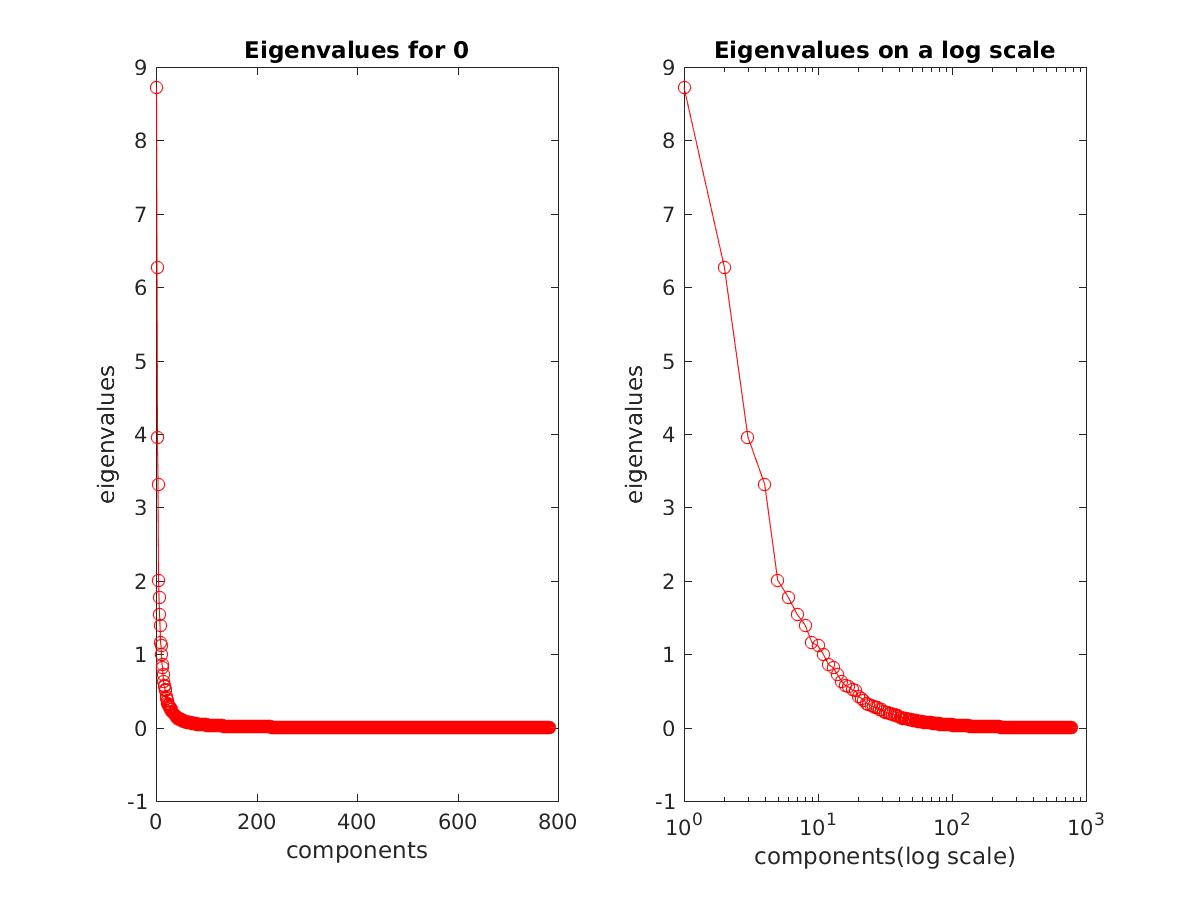
\includegraphics[width=\textwidth, height = 0.25\paperheight]{Eigen_0}
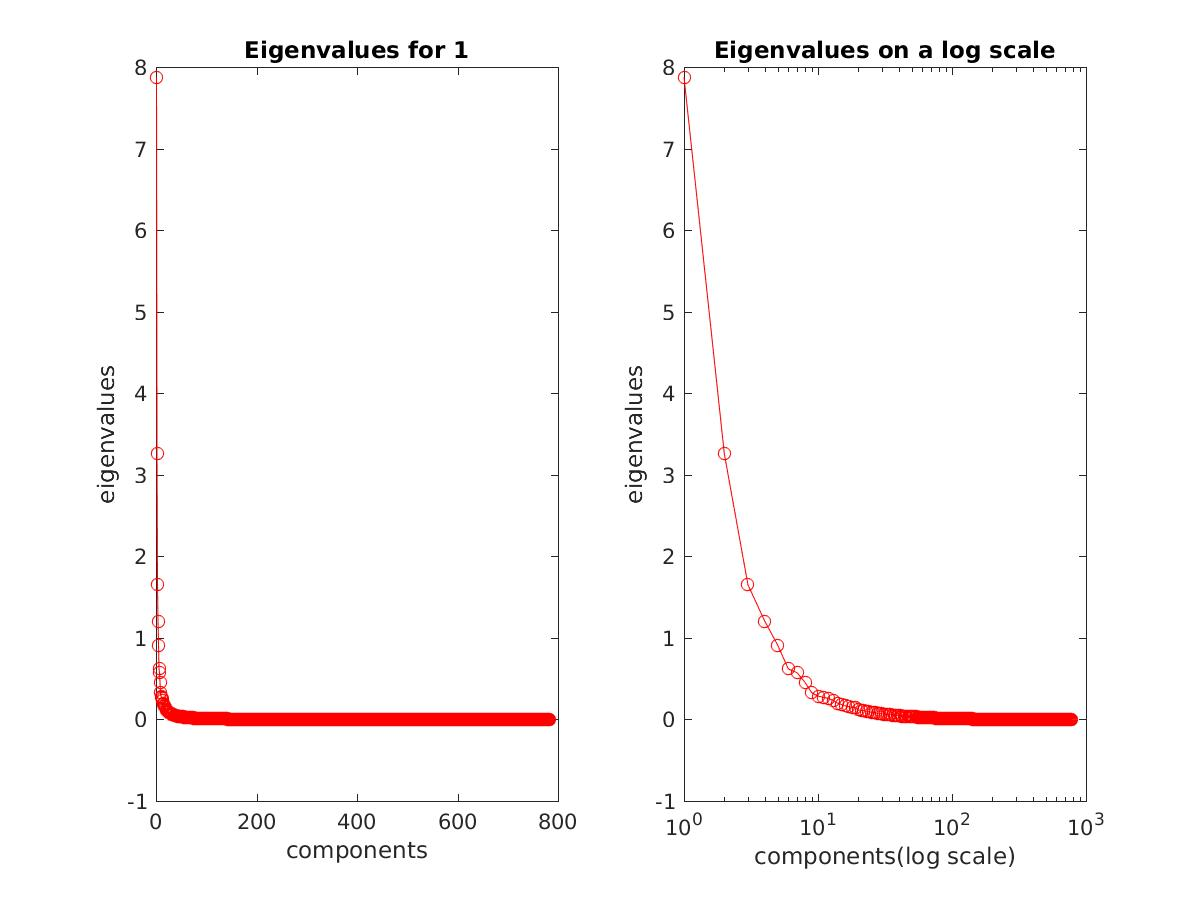
\includegraphics[width=\textwidth, height = 0.25\paperheight]{Eigen_1}
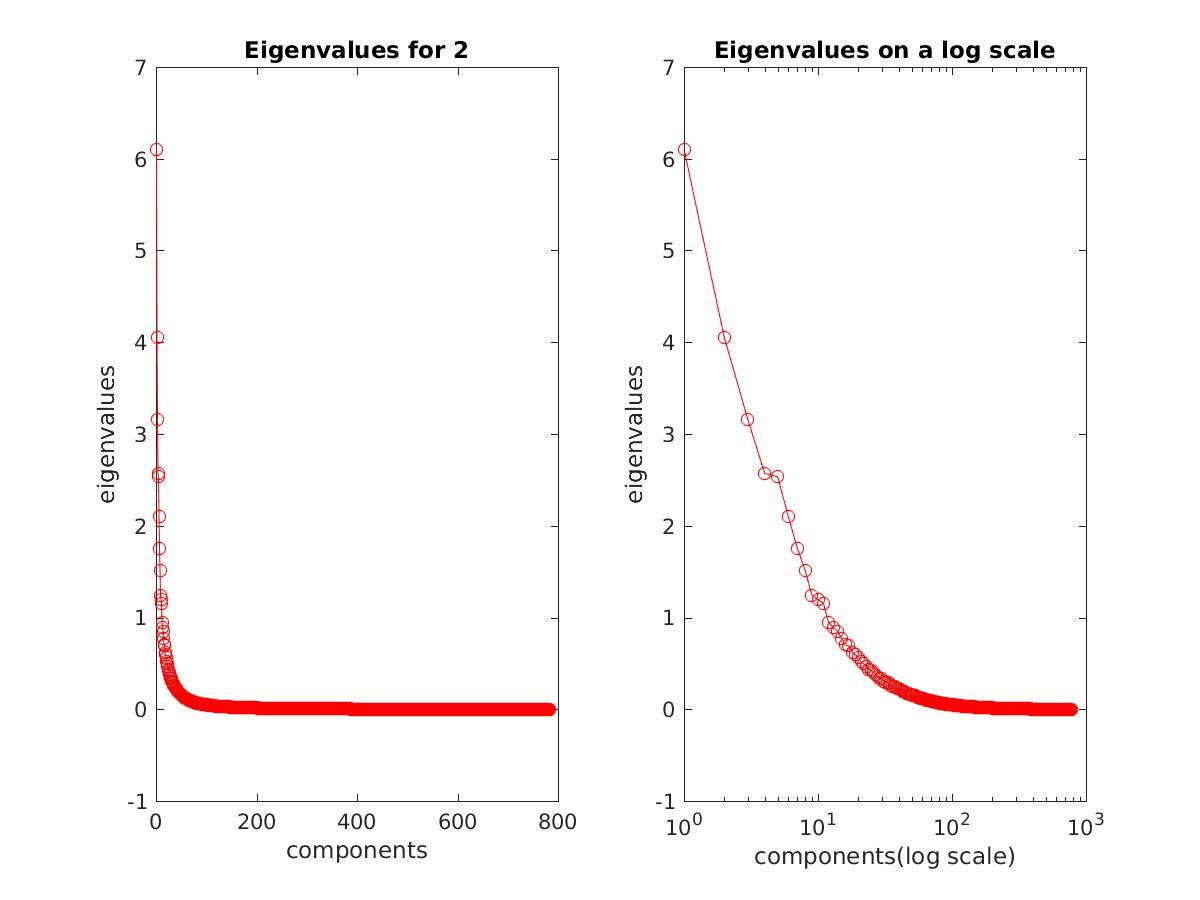
\includegraphics[width=\textwidth, height = 0.25\paperheight]{Eigen_2}
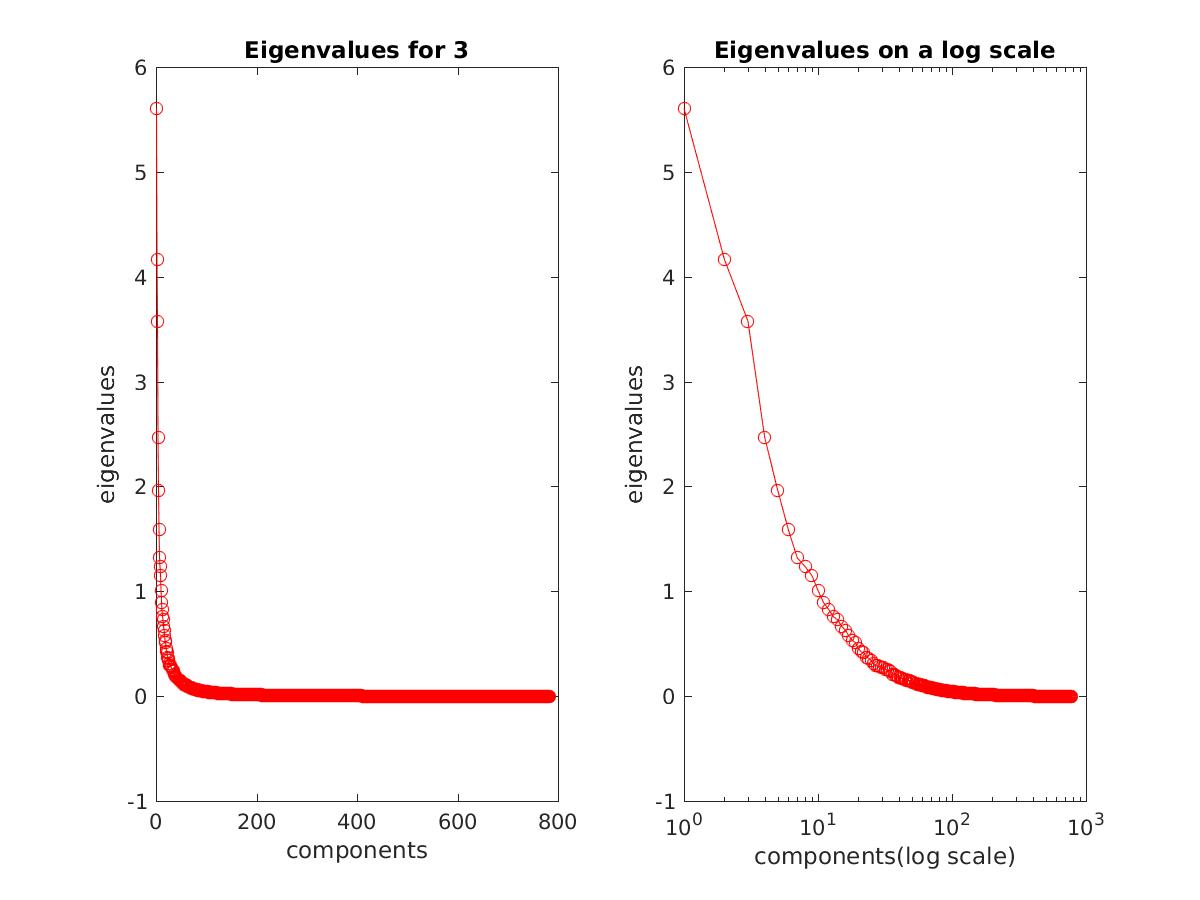
\includegraphics[width=\textwidth, height = 0.25\paperheight]{Eigen_3}
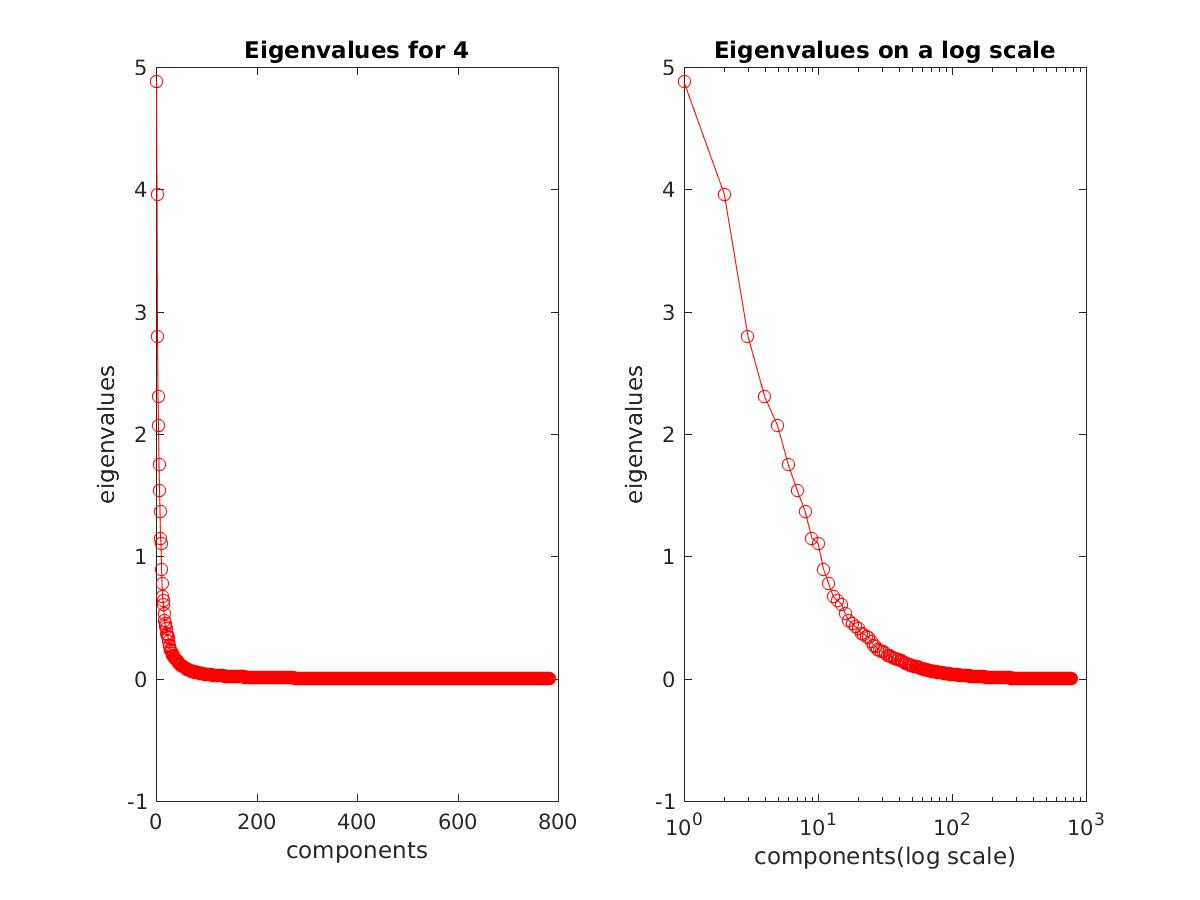
\includegraphics[width=\textwidth, height = 0.25\paperheight]{Eigen_4}
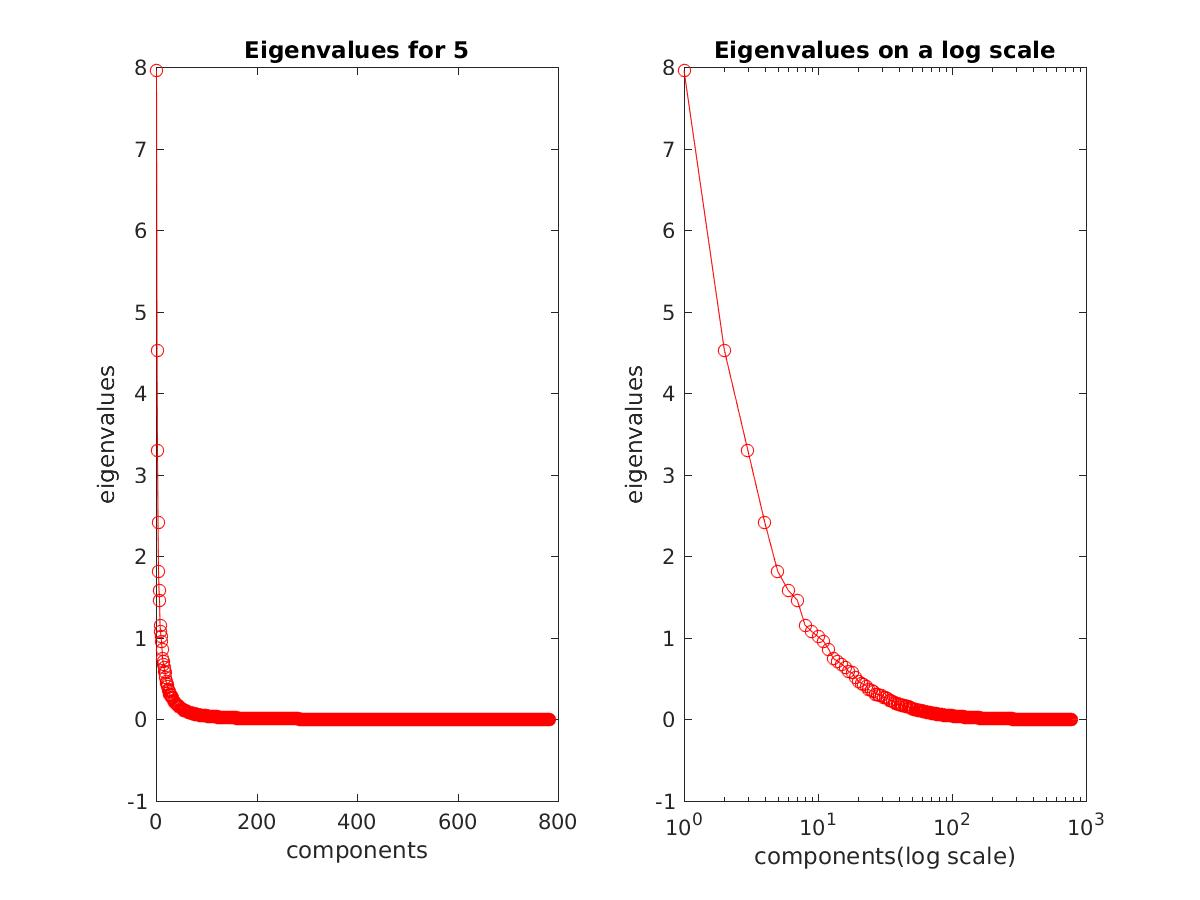
\includegraphics[width=\textwidth, height = 0.25\paperheight]{Eigen_5}
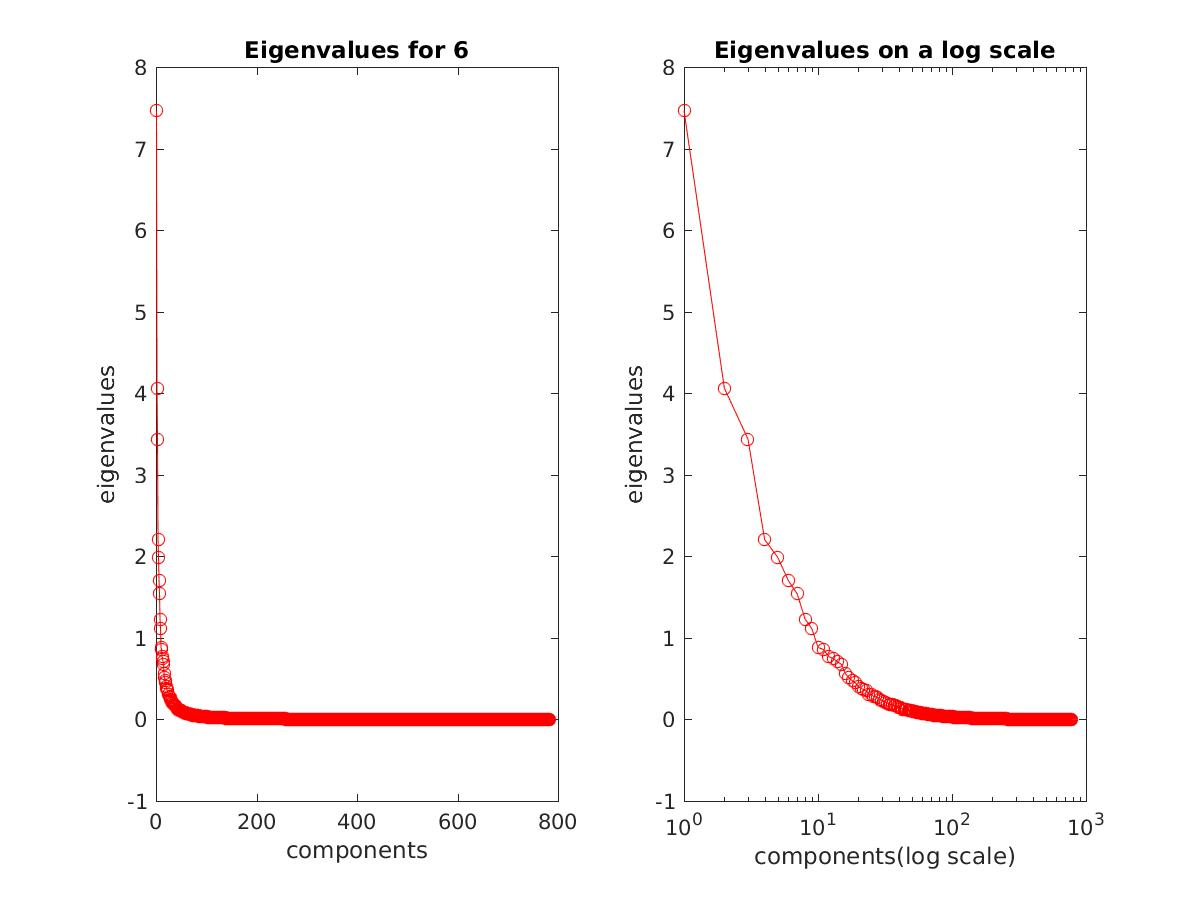
\includegraphics[width=\textwidth, height = 0.25\paperheight]{Eigen_6}
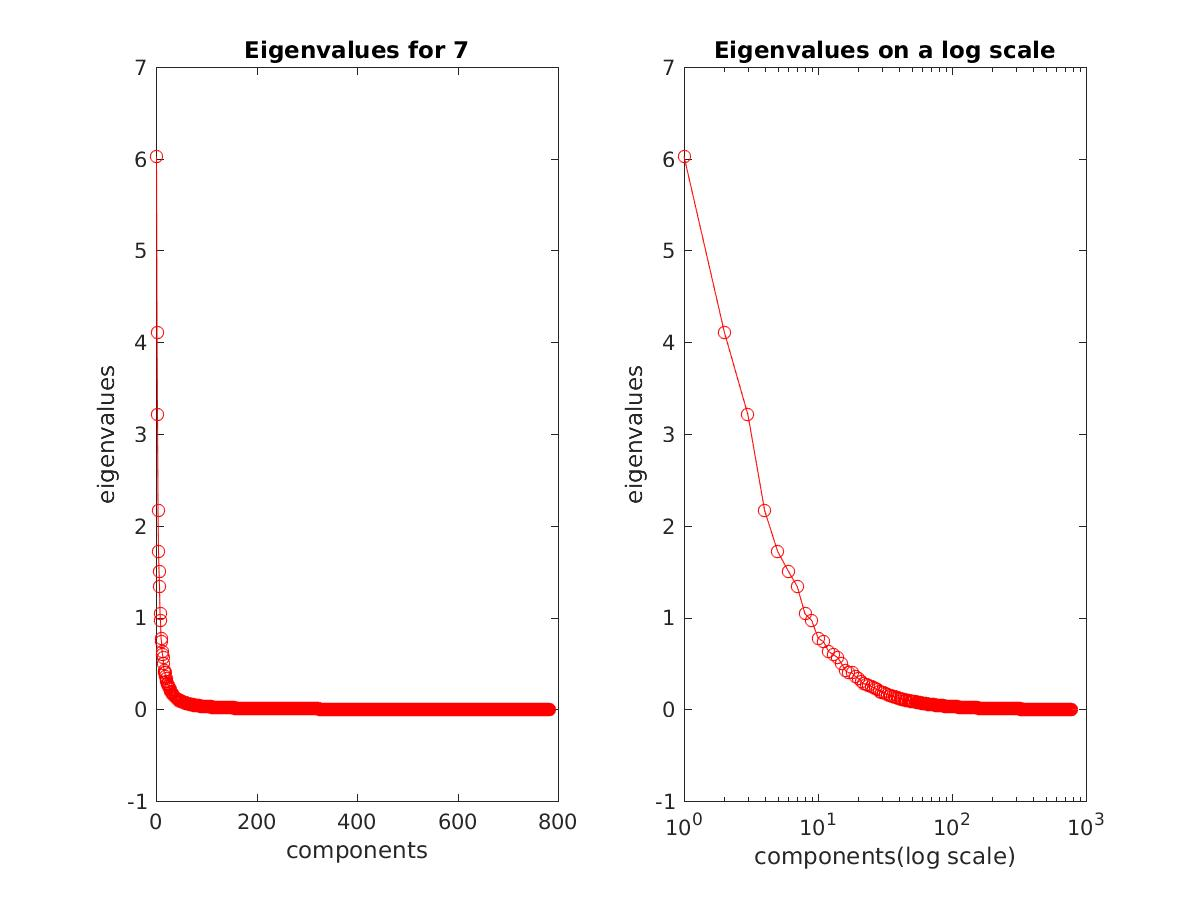
\includegraphics[width=\textwidth, height = 0.25\paperheight]{Eigen_7}
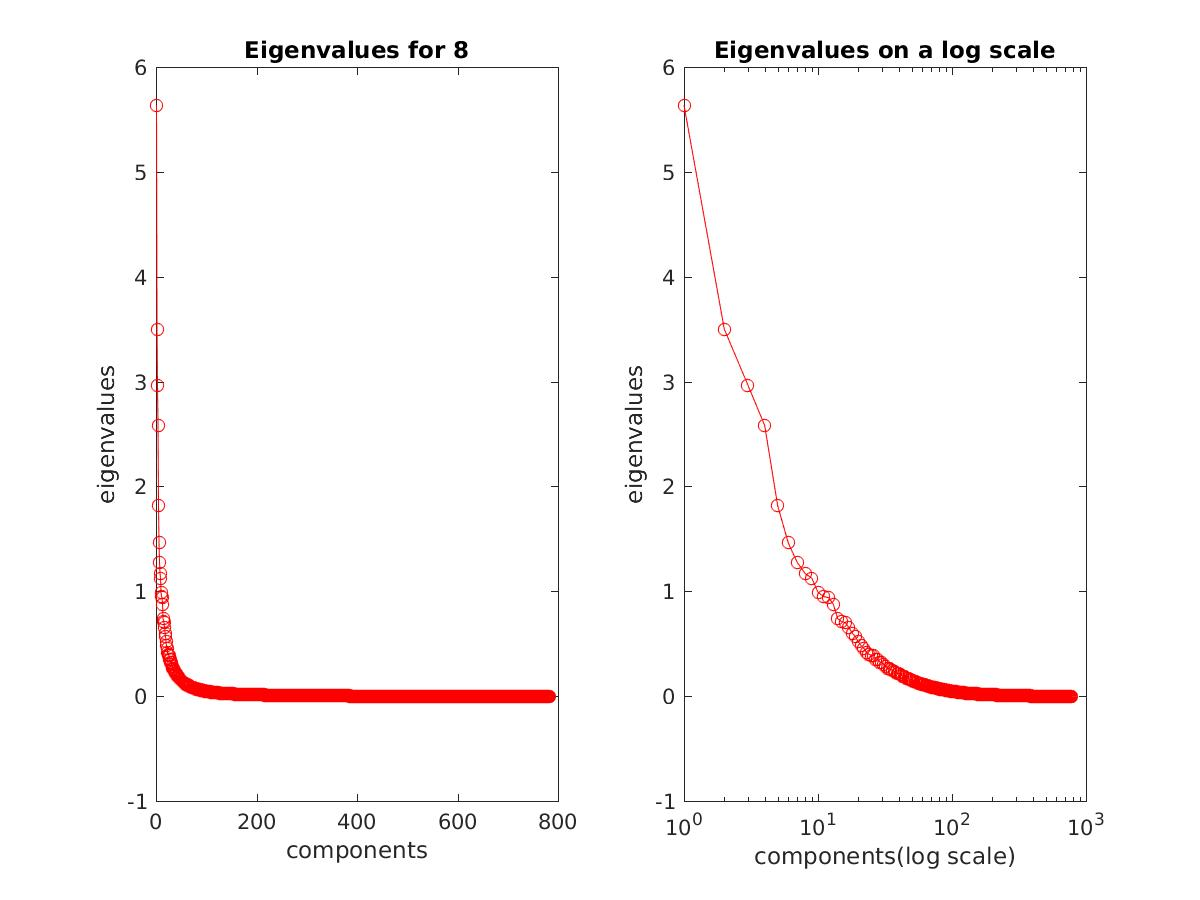
\includegraphics[width=\textwidth, height = 0.25\paperheight]{Eigen_8}
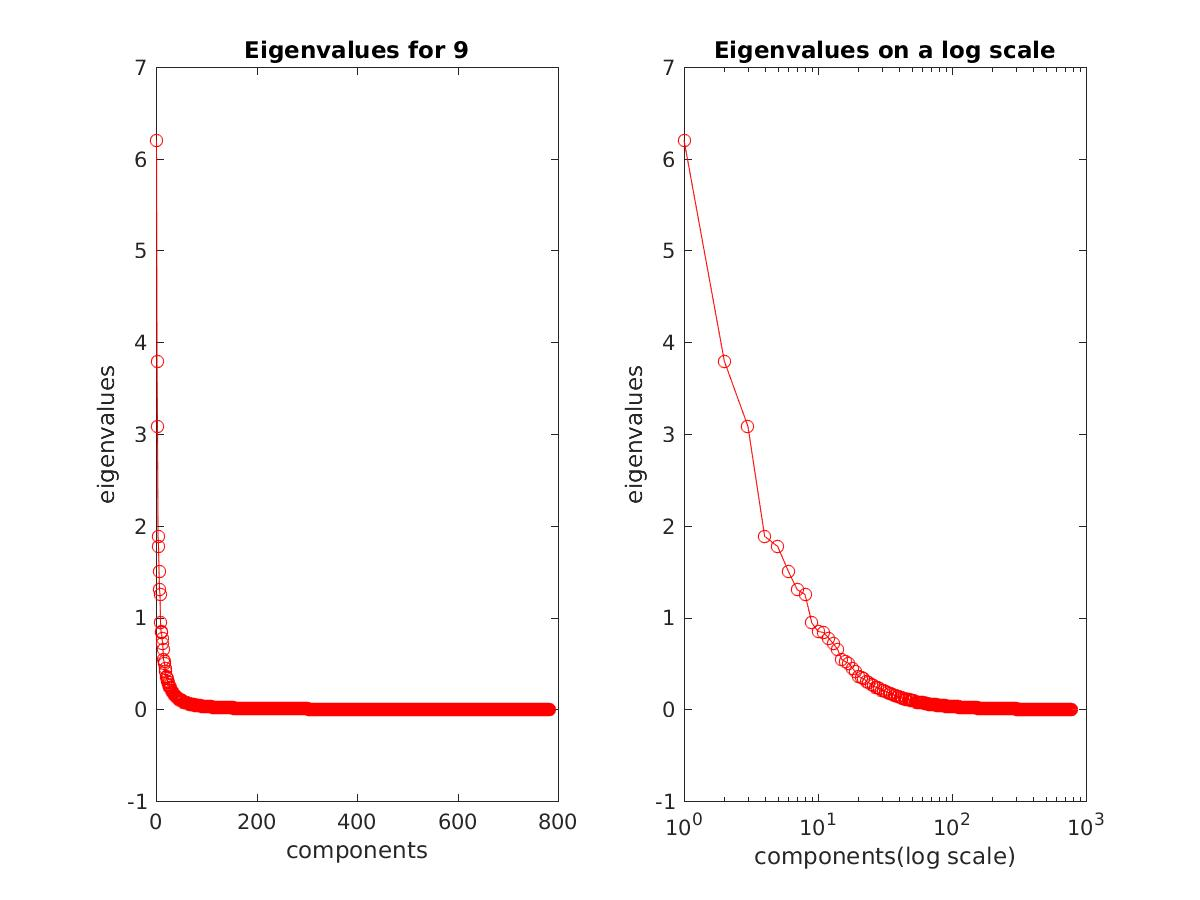
\includegraphics[width=\textwidth, height = 0.25\paperheight]{Eigen_9}

\newpage
\subsection*{4.3 : Part C}
 For every digit, the graph of $\mu - \sqrt{\lambda_1}.v_1$, $\mu$ and $\mu + \sqrt{\lambda_1}.v_1$ was plotted and the following inferences were made:
 \begin{itemize}
 \item The plots plot of \textbf{$\mu$} shows an \textbf{average spread} of the way people usually write the digit.
 \item As discussed earlier, the eigenvector corresponding to the maximum eigenvalue is the \textbf{principle mode of variation}. This is the drection in which the \textbf{variance 'varies' the most}.
 \item We can say that this \textbf{eigenvector} is a \textbf{linear combination} of the 784 variables of our image in a way such that it gives the most significant distinction in data. This obtained feature can be called the \textbf{most optimum} feature.
 \item Hence, $\mu - \sqrt{\lambda_1}v_1$ and $\mu + \sqrt{\lambda_1}.v_1$ will represent a (sort of) \textbf{range} in which \textbf{people usually} will \textbf{write} the respective digit, and if any input data lies within this range, then it will be highly probable that the input data matches this digit.
 \item For intance, in the case of the digit one, we observe two oblique lines in the two plots. This implies that the digit one, which ideally is a standing line, can be given some margin of error, and allow the user to write a 'one' with a slight slanting line as well.
 \end{itemize}
 
 \noindent The plots of the comparison follow:
 
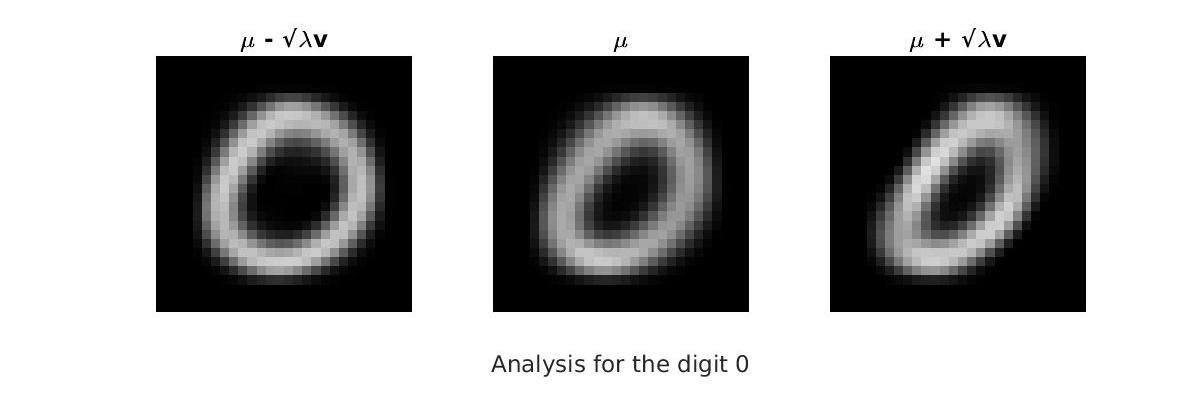
\includegraphics[width=\textwidth, height = 0.25\paperheight]{Comparison_mu_0}
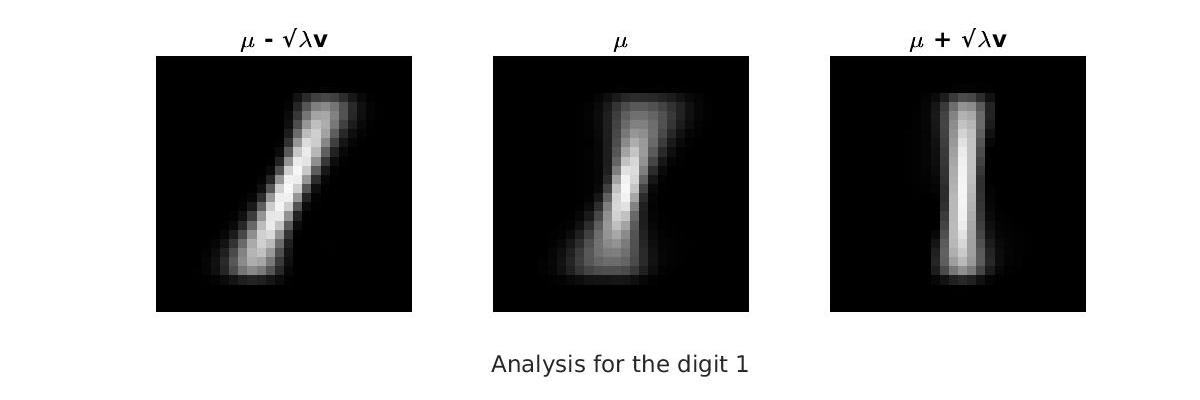
\includegraphics[width=\textwidth, height = 0.25\paperheight]{Comparison_mu_1}
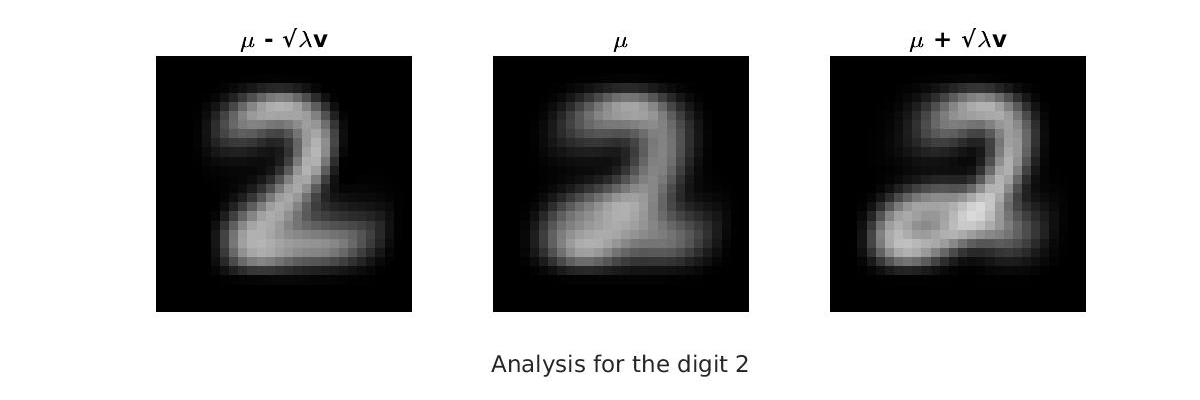
\includegraphics[width=\textwidth, height = 0.25\paperheight]{Comparison_mu_2}
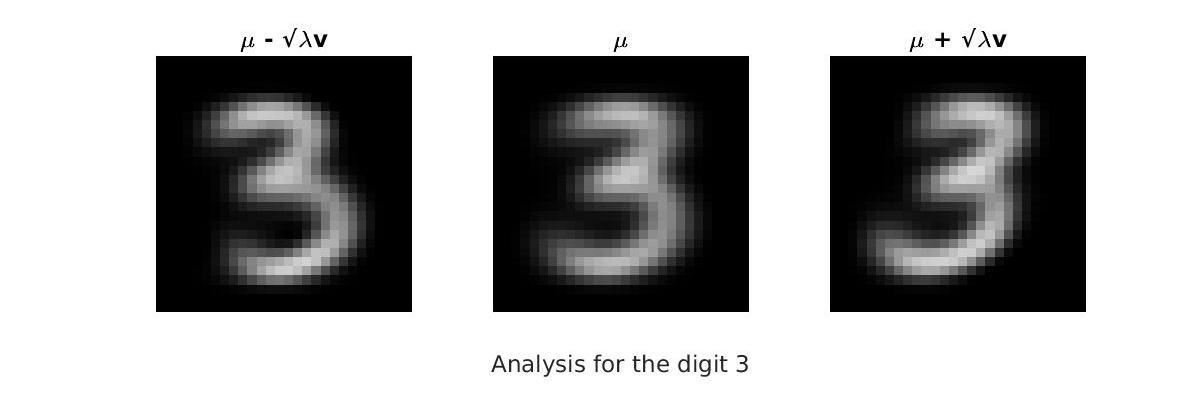
\includegraphics[width=\textwidth, height = 0.25\paperheight]{Comparison_mu_3}
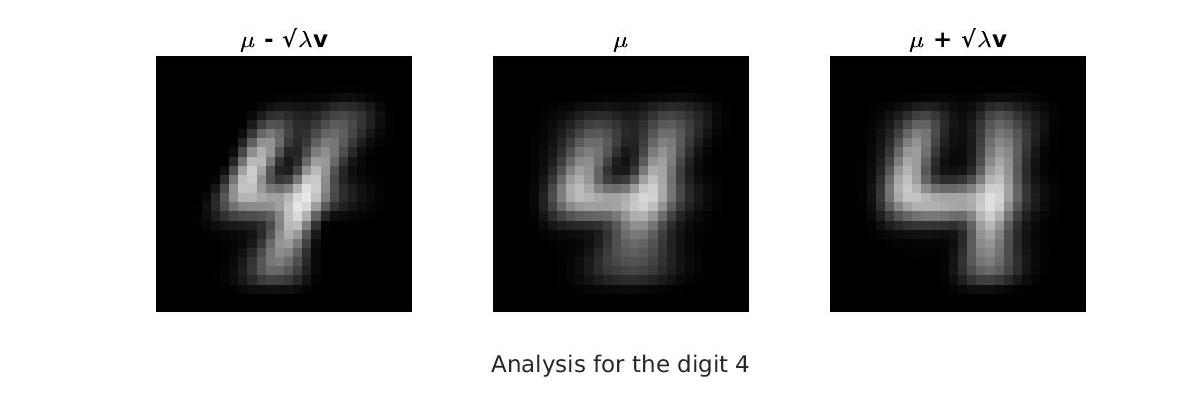
\includegraphics[width=\textwidth, height = 0.25\paperheight]{Comparison_mu_4}
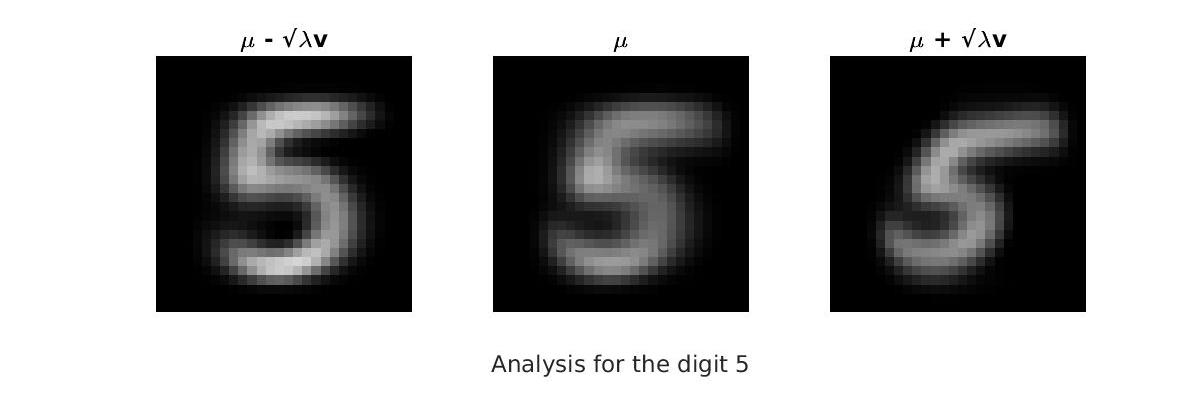
\includegraphics[width=\textwidth, height = 0.25\paperheight]{Comparison_mu_5}
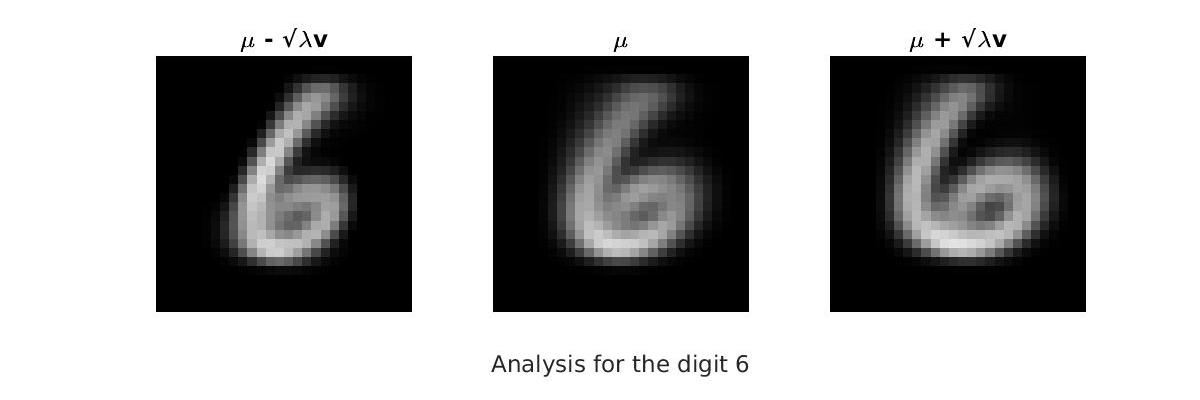
\includegraphics[width=\textwidth, height = 0.25\paperheight]{Comparison_mu_6}
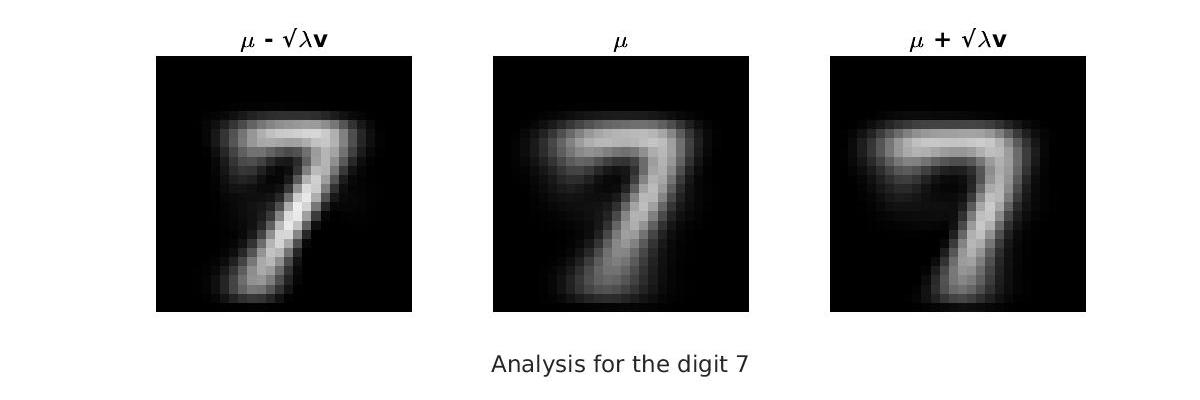
\includegraphics[width=\textwidth, height = 0.25\paperheight]{Comparison_mu_7}
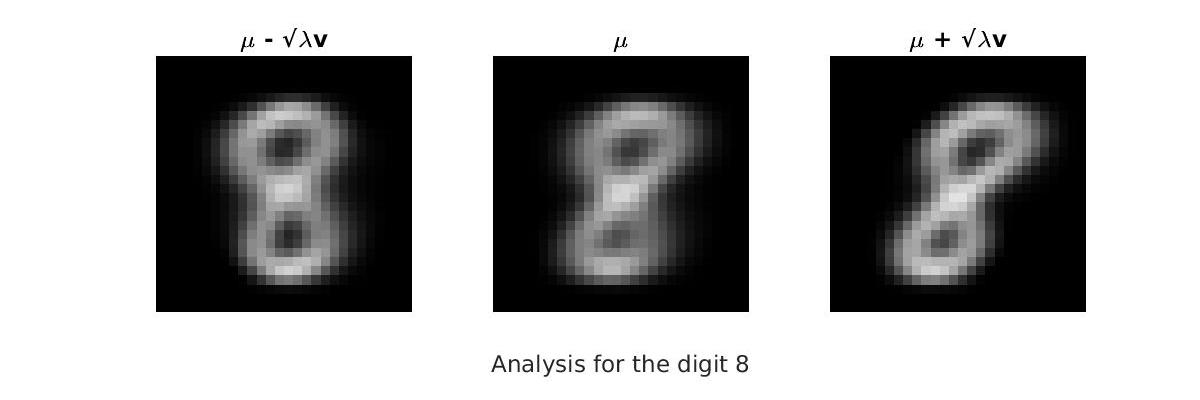
\includegraphics[width=\textwidth, height = 0.25\paperheight]{Comparison_mu_8}
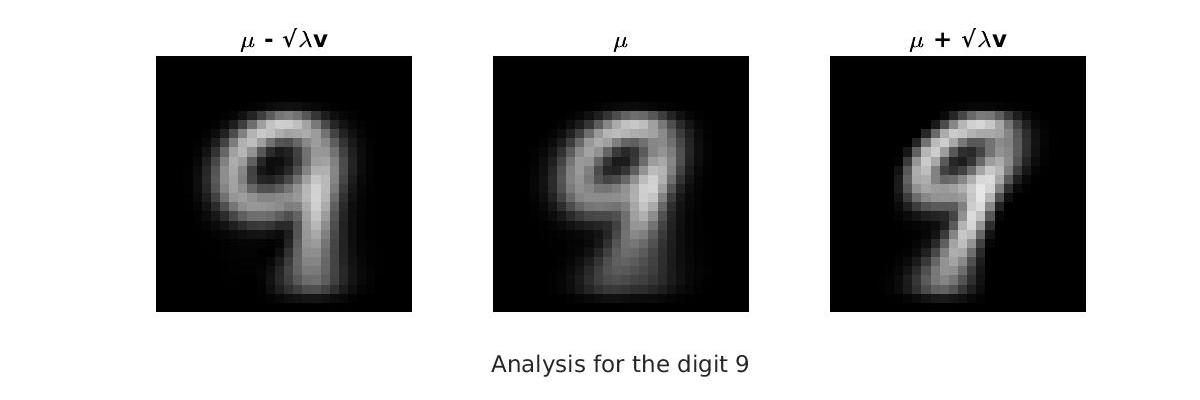
\includegraphics[width=\textwidth, height = 0.25\paperheight]{Comparison_mu_9} 
 
 \newpage
\subsection*{4.4 : Usage of Code}
The following are the instructions for the usage of the code:
\begin{itemize}
\item Load the code present in \lq submission/code/q4/q4.m \rq \space.
\item In the same directory are functions implemented like myMean, myCov which return the mean and covariance of appropriate matrices.
\item Simply run the code in \lq q4.m \rq \space and this wil automatically create the required plots.
\item Lines 44, 58 (commented by default) hava a code to save jpg files of the respective plots. Comment/Uncomment these lines appropriately according to need.
\item The results.mat present in \lq results/mat\rq \space contains all the required results for the partA stored: 
	\begin{description}
	\item[Mean Vectors:] Stored as a cell by the name MeanVectors, where the ith cell has the mean vector for the digit \lq i\rq
	\item[Covariance Matrix:] Stored as a cell by the name CovarianceMatrices, where the ith cell has the Covariance Matrix for the digit \lq i\rq
	\item[First Modes of Variation:] Stored as a cell by the name FirstModesOfVariation, where the ith cell has the First Mode of Variation for the digit \lq i\rq
	\item[Maximum Eigenvalues:] Stored as a cell by the name MaxEigenValues, where the ith cell has the Maximum Eigenvalue for the digit \lq i\rq
	\end{description}

\end{itemize}
 
 
\end{document}